% Copyright 2026 Sreeram Anil
% SPDX-License-Identifier: CC-BY-4.0
\chapter{Ensemble Kalman filter (EnKF)}
\label{ch:enkf}

\section*{At a glance}
\begin{tabular}{@{}l>{\raggedright\arraybackslash}p{0.76\textwidth}@{}}
Family & Sequential Monte Carlo (particle / ensemble / Gaussian sum) \\
Header & \texttt{include/estkit/particle/enkf.hpp} \\
Registered name & \texttt{EnKF} ($N=50$ members, perturbed observations) \\
State dimension & $n_x = 4$ (cell model) — generic in $n_x, n_u, n_y$ \\
Cost per step & \SI{10.3}{\micro\second}/step ($22\times$ EKF); $\mathcal{O}(N(c_f+c_h+n_xn_y)+n_y^3)$ \\
Memory & \SI{6.8}{\kilo\byte} (one $N\times n_x$ ensemble, no $n_x\times n_x$ propagation) \\
Primary references & \cite{evensen1994,burgers1998,evensen2003,anderson1999inflation} \\
\end{tabular}

\section{Motivation and aerospace/BMS relevance}
The extended Kalman filter propagates a covariance matrix through a linearisation; the unscented
filter propagates $2n_x+1$ deterministic points through the true dynamics; the ensemble Kalman
filter propagates $N$ \emph{random} points through the true dynamics and reads the covariance off
the sample.  Evensen \cite{evensen1994} introduced it because the alternative was impossible: in
ocean and atmosphere assimilation $n_x$ is $10^7$ to $10^9$, so an $n_x\times n_x$ covariance can
neither be stored nor propagated, whereas an ensemble of $N\sim 100$ model states can.  The EnKF
is the reason modern numerical weather prediction has uncertainty estimates at all.

For $n_x = 4$ that motivation evaporates --- an EKF covariance is sixteen numbers --- and the EnKF
becomes something else: a Monte-Carlo audit of the Kalman assumptions that needs no Jacobians.
Three properties keep it interesting for a BMS:
\begin{enumerate}[label=(\roman*),leftmargin=2.5em]
  \item it is \emph{derivative-free} --- $\mH$ never appears, only the ensemble in observation
        space, so an OCV curve given as a lookup table with a discontinuous slope (exactly what
        \code{OcvTable} is) causes no trouble at all;
  \item the ensemble travels through the \emph{true} nonlinear map, so the forecast spread
        inherits the real nonlinearity rather than a first-order image of it;
  \item cost and memory scale linearly in $n_x$, which matters for the pack-level and
        joint state/parameter versions of the problem where $n_x$ runs into the hundreds.
\end{enumerate}
Unlike a particle filter, the EnKF is \emph{not} a consistent approximation of the Bayesian
posterior: its analysis step is a linear-Gaussian update.  It approximates the Kalman filter, not
Bayes' rule.  That is worth stating plainly, because it explains why the EnKF sits between the
Kalman family and the particle family in every table in this report.

\section{Problem statement and assumptions}
Model \eqref{eq:pfb-dyn}--\eqref{eq:pfb-meas} again.  The EnKF additionally assumes
\begin{quote}
(A6) the forecast distribution is adequately described by its first two moments, and the analysis
may be performed with a linear gain --- i.e.\ the same assumption as the Kalman filter, applied to
a sample-based covariance.
\end{quote}
It does \emph{not} assume differentiability of $f$ or $h$, and it does not require $\mQ$ or $\mR$
in factored form beyond the ability to sample from them.

\section{Derivation}

\subsection{Forecast}
Every member is integrated through the true dynamics with an independent draw of the process noise,
\begin{equation}
  \vx^{f,i}_k = f\big(\vx^{a,i}_{k-1}, \vu_{k-1}\big) + \vw^i, \qquad
  \vw^i \sim \N{\bm 0}{\mQ}, \qquad i = 1,\dots,N,
  \label{eq:enkf-forecast}
\end{equation}
and the forecast statistics are the sample mean and the (scaled) perturbation matrix
\begin{equation}
  \bar{\vx}^f = \frac1N\sum_i \vx^{f,i}, \qquad
  \bm{X}' = \frac{1}{\sqrt{N-1}}\big[\vx^{f,1}-\bar{\vx}^f,\ \dots,\ \vx^{f,N}-\bar{\vx}^f\big] \in \real^{n_x\times N},
  \label{eq:enkf-Xp}
\end{equation}
so that $\mP^f = \bm{X}'(\bm{X}')^\T$ without ever forming $\bm{X}'(\bm{X}')^\T$ explicitly.

\subsection{Analysis in observation space}
Map the ensemble through the measurement function and form the same quantities there:
\begin{equation}
  \vy^i = h(\vx^{f,i},\vu_k), \qquad \bar{\vy} = \frac1N\sum_i \vy^i, \qquad
  \bm{Y}' = \frac{1}{\sqrt{N-1}}\big[\vy^1-\bar{\vy},\dots,\vy^N-\bar{\vy}\big] \in \real^{n_y\times N}.
  \label{eq:enkf-Yp}
\end{equation}
The cross- and innovation covariances and the gain follow as sample estimates,
\begin{equation}
  \mP_{xy} = \bm{X}'(\bm{Y}')^\T, \qquad
  \mP_{yy} = \bm{Y}'(\bm{Y}')^\T + \mR, \qquad
  \mK = \mP_{xy}\,\mP_{yy}\inv .
  \label{eq:enkf-K}
\end{equation}
Comparing with the Kalman gain $\mP^f\mH^\T(\mH\mP^f\mH^\T+\mR)\inv$ shows that $\bm{X}'(\bm{Y}')^\T$ has
taken the place of $\mP^f\mH^\T$: the Jacobian has been replaced by a sample covariance between the
state and observation ensembles, which for a linear $h$ is exactly equal and for a nonlinear $h$ is
a statistical linearisation over the actual forecast spread.

\subsection{Perturbed observations: why they are not optional}
The naive analysis $\vx^{a,i} = \vx^{f,i} + \mK(\vy_k - \vy^i)$ updates every member with the
\emph{same} measurement.  Burgers, van Leeuwen and Evensen \cite{burgers1998} showed that the
resulting analysis ensemble is systematically under-dispersed.  Writing
$\bm{X}'_a = (\mI - \mK\mH)\bm{X}'$ for the linear case gives
\begin{equation}
  \mP^a_{\text{naive}} = (\mI-\mK\mH)\mP^f(\mI-\mK\mH)^\T
  = (\mI-\mK\mH)\mP^f - \mK\mR\mK^\T ,
  \label{eq:enkf-naive}
\end{equation}
which is short of the correct Kalman analysis covariance $(\mI - \mK\mH)\mP^f$ by exactly the term
$\mK\mR\mK^\T$.  The deficit compounds over cycles: the ensemble becomes over-confident, the gain
shrinks, the filter stops listening to the data and diverges.  The cure is to give every member its
own realisation of the measurement noise,
\begin{equation}
  \boxed{\;
  \vx^{a,i}_k = \vx^{f,i}_k + \mK\big(\vy_k + \vv^i - \vy^i\big), \qquad \vv^i\sim\N{\bm 0}{\mR}\;}
  \label{eq:enkf-analysis}
\end{equation}
so that $\E{\mP^a} = (\mI-\mK\mH)\mP^f$ exactly, as in the Kalman filter.  The perturbations are
centred, $\sum_i \vv^i = \bm 0$, which removes the leading-order sampling error without biasing the
spread \cite[\S4.3]{evensen2003}.

\subsection{Covariance inflation}
Two effects make a finite ensemble under-disperse in practice: sampling error in $\mK$ (order
$N^{-1/2}$) and the absence of any representation of model error beyond $\mQ$.  The standard remedy
\cite{anderson1999inflation} is multiplicative inflation of the forecast perturbations about their
mean,
\begin{equation}
  \vx^{f,i} \leftarrow \bar{\vx}^f + \rho\,\big(\vx^{f,i} - \bar{\vx}^f\big), \qquad \rho \ge 1,
  \label{eq:enkf-inflation}
\end{equation}
applied before the analysis.  Inflation is a \emph{per-cycle} correction, so its numerical value
depends on the assimilation rate: the values $\rho \in [1.01, 1.05]$ quoted in the meteorological
literature refer to cycles hours apart.  At \SI{10}{\hertz} the same factor compounds
$\num{20100}$ times over one eVTOL mission.  The quantitative effect on the steady-state spread
follows from balancing inflation against the analysis contraction: with a scalar measurement,
$\rho^2(1 - KH) = 1$ gives $KH = 1-\rho^{-2}$, hence
\begin{equation}
  \mP_{\soc\soc}\,H^2 \;\approx\; (\rho^2-1)\,\mR
  \label{eq:enkf-inflation-balance}
\end{equation}
as the floor that inflation puts under the ensemble variance.  With $\rho = 1.001$ and the cell's
numbers this is $\sqrt{\mP_{\soc\soc}} \approx 3\times10^{-4}$ --- small enough not to disturb the
estimate, large enough to keep the gain alive.  Section~\ref{sec:enkf-battery} reports the measured
sweep.

\section{Algorithm}
\begin{algorithm}[H]
\caption{EnKF (stochastic, perturbed observations) --- one sampling period}
\begin{algorithmic}[1]
\Require ensemble $\{\vx^{a,i}_{k-1}\}_{i=1}^N$, $\vu_{k-1},\vu_k,\vy_k$
\State \textbf{Forecast.} $\mL_Q \gets \operatorname{chol}(\mQ(\xhat_{k-1},\vu_{k-1}))$
\For{$i=1$ \textbf{to} $N$} \State $\vx^{f,i} \gets \operatorname{constrain}\big(f(\vx^{a,i}_{k-1},\vu_{k-1}) + \mL_Q\bm\xi^i\big)$ \EndFor
\State \textbf{Prior predictive.} $\yhat_k \gets \frac1N\sum_i h(\vx^{f,i},\vu_k)$
\State \textbf{Inflation.} $\bar{\vx}^f \gets \frac1N\sum_i \vx^{f,i}$; \; $\vx^{f,i}\gets \bar{\vx}^f + \rho(\vx^{f,i}-\bar{\vx}^f)$
\State \textbf{Observation ensemble.} $\vy^i \gets h(\vx^{f,i},\vu_k)$; \; $\bar{\vy}\gets\frac1N\sum_i\vy^i$
\State $\mP_{xy} \gets \frac{1}{N-1}\sum_i (\vx^{f,i}-\bar{\vx}^f)(\vy^i-\bar{\vy})^\T$
\State $\mP_{yy} \gets \mR + \frac{1}{N-1}\sum_i (\vy^i-\bar{\vy})(\vy^i-\bar{\vy})^\T$; \quad $\mK \gets \mP_{xy}\mP_{yy}\inv$
\State \textbf{Perturbations.} $\vv^i \gets \mL_R\bm\eta^i$, $\bm\eta^i\sim\N{\bm 0}{\mI}$; \; $\vv^i \gets \vv^i - \frac1N\sum_m \vv^m$
\For{$i=1$ \textbf{to} $N$} \State $\vx^{a,i} \gets \operatorname{constrain}\big(\vx^{f,i} + \mK(\vy_k + \vv^i - \vy^i)\big)$ \EndFor
\State $\xhat_k \gets \frac1N\sum_i \vx^{a,i}$; \quad $\mP_k \gets \frac{1}{N-1}\sum_i (\vx^{a,i}-\xhat_k)(\vx^{a,i}-\xhat_k)^\T$
\Ensure $\xhat_k$, $\mP_k$, analysis ensemble
\end{algorithmic}
\end{algorithm}

\section{Application to the battery model}
\label{sec:enkf-battery}
With $n_y = 1$ the analysis is scalar: $\mP_{yy}$ is a number, $\mK$ is a $4\times1$ vector, and the
whole update costs $N(n_x + 2)$ multiply-adds after the $N$ evaluations of $f$ and $h$.  The
ensemble in observation space is the set of terminal voltages the $N$ cell replicas would produce,
which is the most physically transparent object in this entire family: its spread \emph{is} the
filter's predicted voltage uncertainty.

\paragraph{Inflation is the one tuning decision.}  Steady-state SOC RMSE in \% over the eVTOL
mission, development run, seed 1 (the final three-seed numbers for the shipped $\rho$ are in the
table of Section~\ref{sec:enkf-results}):
\begin{center}
\begin{tabular}{@{}lccccc@{}}
\toprule
$\rho$ & 1 & 1.0005 & 1.001 & 1.002 & 1.005 \\
\midrule
\code{nominal}        & 0.19 & 0.09 & 0.28 & 0.36 & 1.50 \\
\code{init\_error}    & 3.25$^\dagger$ & 2.93$^\dagger$ & 0.28 & 0.36 & 1.61 \\
\code{current\_bias}  & 2.04 & 1.48 & 0.81 & 1.18 & 1.77 \\
\code{param\_mismatch}& 1.14 & 2.32 & 2.15 & 3.24 & 4.97 \\
\bottomrule
\end{tabular}
\end{center}
\noindent ($^\dagger$ never reaches the \SI{2}{\percent} convergence band.)  Without inflation the
ensemble collapses after the first large correction and cannot recover a \SI{35}{\percent}
initialisation error at all; above $\rho = 1.002$ the compounding at \SI{10}{\hertz} inflates the
weakly observable SOC--$v_2$ direction faster than the measurement contracts it, and accuracy
degrades in every scenario.  The default $\rho = 1.001$ --- one part in a thousand per step, i.e.\
\SI{1}{\percent} per second --- is the balance point, and it is the ensemble-filter analogue of the
roughening cap discussed in Section~\ref{sec:pfb-battery}.

\paragraph{Sampling error dominates the transient.}  With $N=50$ the relative error of the sample
gain is $\mathcal{O}(N^{-1/2}) = \SI{14}{\percent}$.  In \code{init\_error} the first analysis
therefore removes only about \SI{85}{\percent} of the \num{0.35} SOC offset, leaving \num{0.06};
the analysis covariance has meanwhile contracted by three orders of magnitude, so the remaining
error is worked off at the slow rate that inflation permits --- \SI{220}{\second}.  The EKF, whose
gain is exact, removes the whole offset in one step.  This is the price of estimating a gain from
50 samples, and it is the single most visible EnKF artefact in the benchmark.

\section{Implementation notes}
\emph{Memory.} \SI{6.8}{\kilo\byte}, the second smallest in the family (after the ETKF) and an
order of magnitude below the particle filters: one $N\times n_x$ ensemble plus two $N$-vectors in
observation space.  No $n_x\times n_x$ matrix is ever propagated; $\mP_k$ is computed only because
the benchmark asks for \code{soc\_std}.

\emph{Cost.} \SI{10.3}{\micro\second}/step, $22\times$ the EKF and $7.4\times$ faster than
\estname{PF-Bootstrap}.  Per step: $N$ evaluations of $f$, $2N$ of $h$, $Nn_x$ Gaussian draws for
$\mQ$, $Nn_y$ for the observation perturbations, and one $n_y\times n_y$ inverse.

\emph{Numerics.}  No logarithms, no exponentials, no weights: the EnKF has none of the dynamic-range
problems of the importance-sampling filters and behaves identically in \code{float32}
($\mathrm{RMSE}_{\mathrm{ss}} = \SI{0.25}{\percent}$ in both precisions on \code{nominal},
Table~\ref{tab:float}).  $\mP_{yy}$ is
inverted with the general \code{inverse()} (a scalar division for $n_y=1$); a rank-deficient
observation ensemble cannot make it singular because $\mR$ is added first.

\emph{Constraints.}  \code{constrain()} is applied after the forecast and after the analysis, so
every member stays a physically realisable cell.  Note that this makes the analysis ensemble
slightly non-Gaussian, which is harmless here but means the reported $\mP_k$ is a sample covariance
of a truncated distribution.

\section{Benchmark results}
\label{sec:enkf-results}
% Copyright 2026 Sreeram Anil
% SPDX-License-Identifier: CC-BY-4.0
\begin{table}[H]\centering\footnotesize\setlength{\tabcolsep}{4pt}
\caption{EnKF: cell-level benchmark on the eVTOL mission (mean over seeds; RMSE and max error in \% SOC; $t_\mathrm{conv}$: first time the error stays below 2\,\% for 60\,s, -- = never; EKF reference: steady-state RMSE of the plain EKF on the same data).}\label{tab:cell_EnKF}
\begin{tabular}{llrrrrrcrr}\toprule
plant & scenario & RMSE & RMSE$_\mathrm{ss}$ & max & $t_\mathrm{conv}$ [s] & RMSE$_v$ [mV] & div. & EKF ref. & ns/step \\ \midrule
ECM & nominal & 0.35 & 0.27 & 3.17 & 0 & 0.82 & no & 0.05 & 10283 \\
ECM & init\_error & 1.50 & 0.27 & 7.44 & 215 & 2.09 & no & 0.05 & 10315 \\
ECM & current\_bias & 0.79 & 0.84 & 2.87 & 0 & 0.86 & no & 0.61 & 10258 \\
ECM & noise\_step & 1.63 & 1.99 & 5.88 & 0 & 2.95 & no & 0.12 & 10358 \\
ECM & outliers & 1.11 & 0.96 & 6.39 & 109 & 2.19 & no & 0.21 & 10307 \\
ECM & cold & 0.86 & 1.07 & 3.36 & 0 & 1.91 & no & 0.16 & 10318 \\
ECM & hot & 0.18 & 0.14 & 3.22 & 0 & 0.59 & no & 0.03 & 10316 \\
ECM & aged\_cell & 4.30 & 2.11 & 14.00 & 349 & 3.58 & no & 1.52 & 10293 \\
ECM & param\_mismatch & 3.60 & 3.58 & 11.51 & 107 & 2.76 & no & 1.36 & 10259 \\
ECM & sensor\_dropout & 1.93 & 0.33 & 7.64 & 0 & 1.78 & no & 0.46 & 10247 \\
ECM & preisach & 1.43 & 1.00 & 5.52 & 215 & 0.85 & no & 0.20 & 10317 \\
ECM & combined & 5.67 & 3.75 & 17.18 & 502 & 4.40 & no & 12.44 & 10191 \\
\midrule
SPM & nominal & 2.31 & 1.67 & 6.14 & 166 & 1.06 & no & 3.73 & 9947 \\
SPM & init\_error & 3.13 & 1.42 & 7.57 & 486 & 2.14 & no & 3.81 & 9960 \\
SPM & current\_bias & 2.38 & 1.88 & 6.19 & 170 & 1.13 & no & 5.69 & 9923 \\
SPM & noise\_step & 8.87 & 11.94 & 19.50 & 166 & 3.21 & no & 3.30 & 10020 \\
SPM & outliers & 10.42 & 13.68 & 22.08 & 62 & 2.42 & no & 1.99 & 10084 \\
SPM & cold & 13.04 & 14.97 & 28.77 & 463 & 4.10 & yes & 7.35 & 10026 \\
SPM & hot & 1.49 & 1.30 & 4.37 & 158 & 0.73 & no & 2.16 & 9983 \\
SPM & param\_mismatch & 8.78 & 8.27 & 14.49 & 495 & 2.02 & no & 3.13 & 9940 \\
SPM & sensor\_dropout & 2.57 & 1.80 & 7.21 & 162 & 1.92 & no & 5.31 & 10070 \\
\bottomrule\end{tabular}\end{table}

\begin{figure}[H]\centering
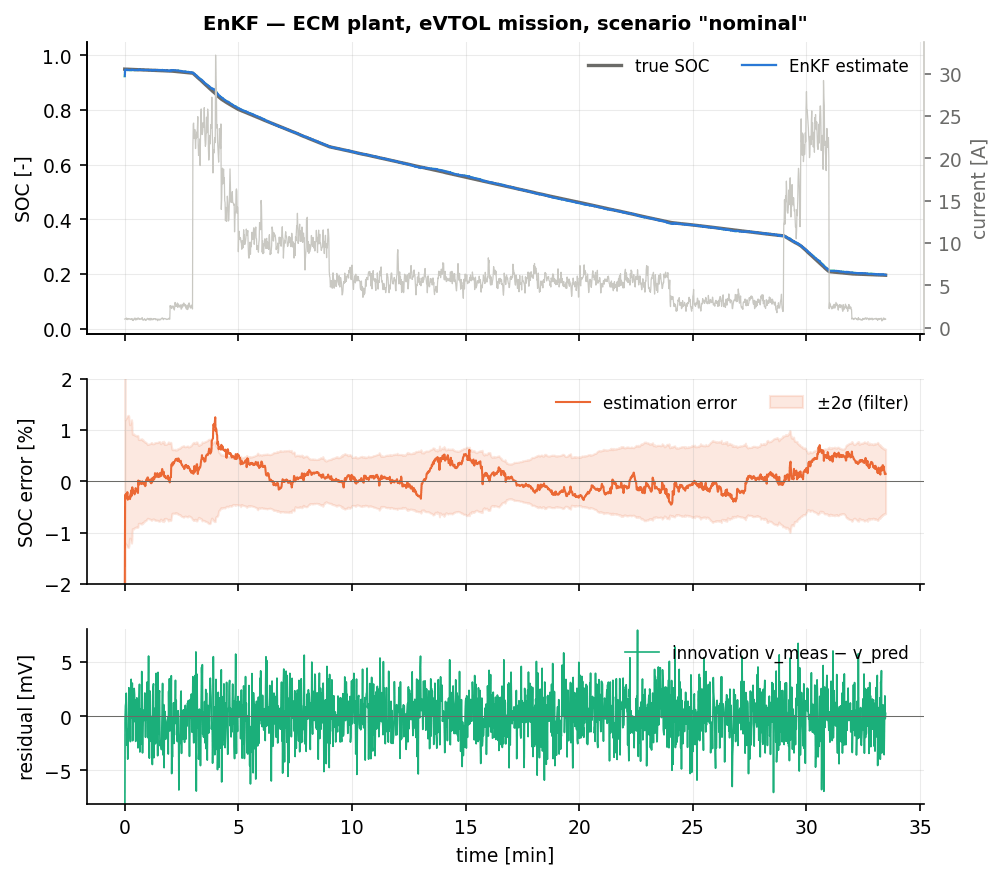
\includegraphics[width=\textwidth]{figures/cell_EnKF_nominal.png}
\caption{EnKF on the nominal eVTOL mission: true and estimated SOC (top), estimation error with the
$\pm2\sigma$ band from the ensemble covariance (middle), voltage residual (bottom).}
\end{figure}
\begin{figure}[H]\centering
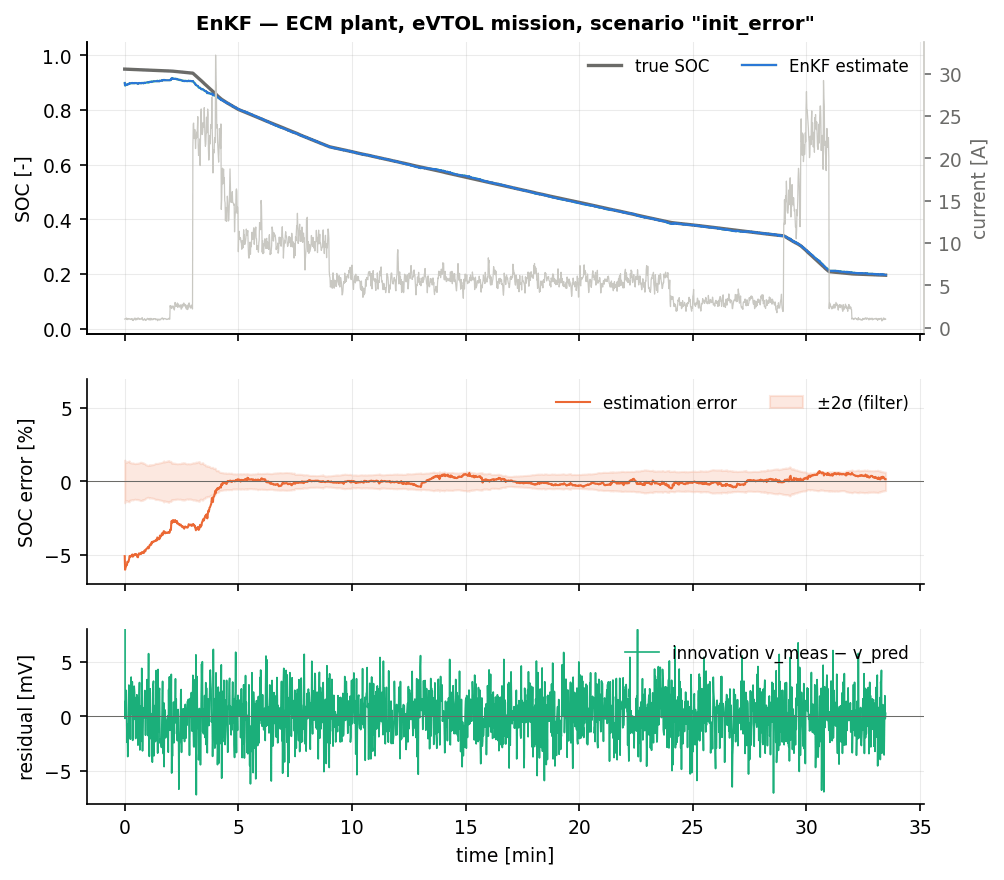
\includegraphics[width=\textwidth]{figures/cell_EnKF_init_error.png}
\caption{EnKF with a \SI{35}{\percent} initial SOC error.  The first analysis removes most of the
offset; the residual left by the \SI{14}{\percent} sampling error of a 50-member gain is worked off
over \SI{215}{\second} at the rate permitted by the inflation.}
\end{figure}
\begin{figure}[H]\centering
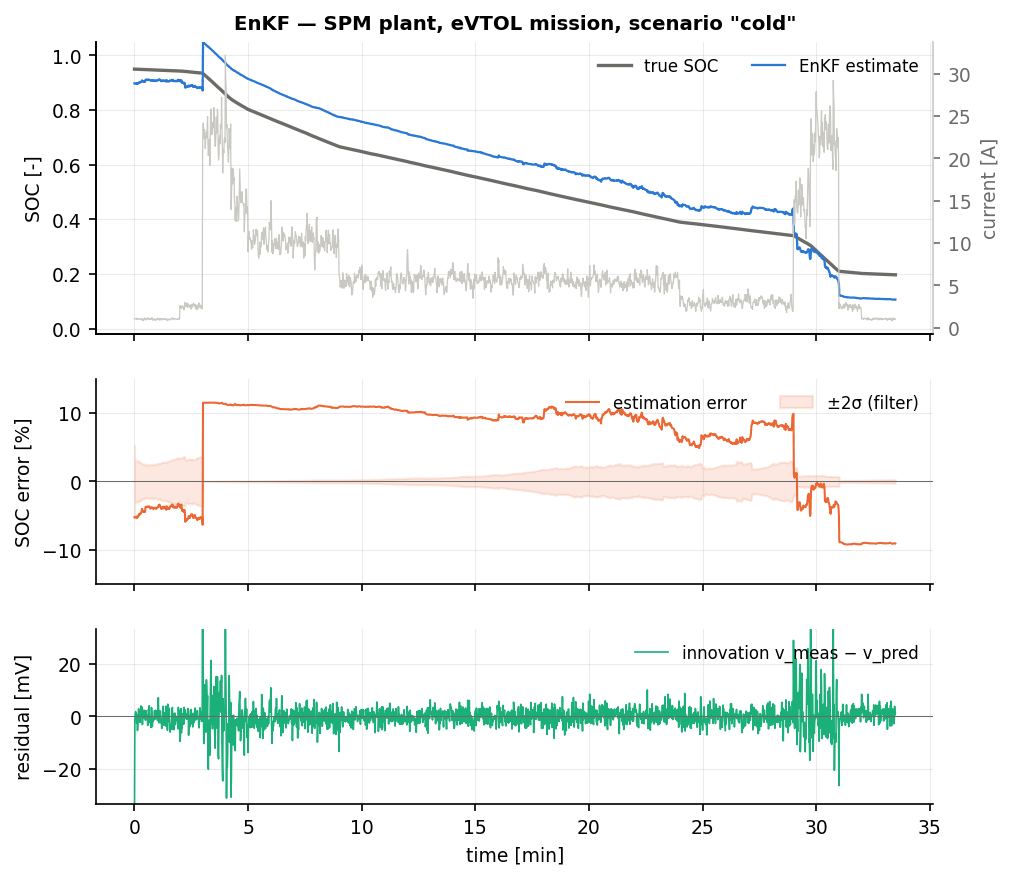
\includegraphics[width=\textwidth]{figures/cellspm_EnKF_cold.png}
\caption{EnKF on the electrochemical (SPM) plant, \code{cold} scenario --- the one divergence of
this family.  At \SI{-10}{\celsius} the SPM's diffusion overpotential grows far beyond what the
fitted 2-RC model can represent, and the stochastic analysis loses the ensemble.}
\end{figure}

\paragraph{ECM plant.}  On \code{nominal} the EnKF reaches $\mathrm{RMSE} = \SI{0.35}{\percent}$,
$\mathrm{RMSE}_{\mathrm{ss}} = \SI{0.27}{\percent}$, maximum error \SI{3.17}{\percent}, immediate
convergence and a voltage-residual RMSE of \SI{0.82}{\milli\volt} --- as good as any Kalman variant
on the voltage residual, and a factor \num{5.4} behind the EKF on SOC (\SI{0.05}{\percent}), which
is the $N^{-1/2}$ sampling penalty one should expect from fifty members.

The scenarios sort themselves along the Kalman/Monte-Carlo divide:
\begin{itemize}[leftmargin=2em]
  \item \textbf{Where the derivative-free forecast helps.}  \code{sensor\_dropout}
        \SI{0.33}{\percent} against \SI{0.46}{\percent} for the EKF and \SI{0.86}{\percent} for the
        UKF; \code{hot} \SI{0.14}{\percent}; \code{aged\_cell} \SI{2.11}{\percent}, the best of the
        two ensemble filters and better than the Gaussian-sum bank (\SI{3.12}{\percent}).  The
        ensemble transported through the true $\ocv$ table captures curvature that a single
        Jacobian misses.
  \item \textbf{Where the sample gain hurts.}  \code{init\_error} needs \SI{215}{\second} to
        converge (steady-state \SI{0.27}{\percent}), and \code{param\_mismatch}
        (\SI{3.58}{\percent} against the EKF's \SI{1.36}{\percent}) and \code{combined}
        (\SI{3.75}{\percent}, converging only after \SI{502}{\second}) are the weakest results of
        the ensemble pair on the ECM plant.  Sampling error in the gain leaves a residual that a
        biased model re-creates faster than the inflated ensemble can remove it.
  \item \code{noise\_step} \SI{1.99}{\percent}, the worst of the family: the fixed $\mR$
        under-states the post-step noise by a factor of ten, and the perturbed observations then
        inject \SI{2}{\milli\volt} perturbations into an ensemble that should be seeing
        \SI{20}{\milli\volt} ones.
  \item \code{preisach} \SI{1.00}{\percent} against the EKF's \SI{0.20}{\percent}: with the
        corrected hysteresis sign convention the unmodelled Preisach loop acts as a slow voltage
        bias, and neither the ensemble spread nor the inflation gives the filter any way to
        attribute it to anything but SOC.
\end{itemize}
Nothing diverges on the ECM plant, and the maximum error over the twelve scenarios is
\SI{17.2}{\percent} (\code{combined}).

\paragraph{SPM plant.}  Against the electrochemical plant the EnKF is the weaker half of a split
verdict.  On \code{nominal} it gives \SI{1.67}{\percent} against the EKF's \SI{3.73}{\percent} --- a
factor \num{2.2}, and far better than the ETKF's \SI{3.82}{\percent} --- and it holds that advantage
on \code{hot} (\SI{1.30}{\percent} against \SI{2.16}{\percent}), \code{current\_bias}
(\SI{1.88}{\percent} against \SI{5.69}{\percent}), \code{sensor\_dropout} (\SI{1.80}{\percent}
against \SI{5.31}{\percent}) and \code{init\_error} (\SI{1.42}{\percent} against
\SI{3.81}{\percent}).  The stochastic forecast, which draws an independent $\mQ$ realisation per
member, plays the same role as the particle filters' roughening: it keeps the ensemble spread in
the $(\soc,v_2)$ direction from collapsing, so the structured \SI{4}{\milli\volt} residual can be
taken up by the RC states instead of by SOC.  That is why the EnKF, alone among the
Gaussian-analysis methods in this family, gets within a factor of three of the particle filters
there.

Its limits are equally clear, and one of them is a divergence.  Three SPM scenarios destroy it:
\code{noise\_step} \SI{11.94}{\percent}, \code{outliers} \SI{13.68}{\percent},
\code{param\_mismatch} \SI{8.27}{\percent}, and \code{cold} \SI{14.97}{\percent} --- \textbf{flagged
as diverged} in the table, the only divergence anywhere in this family.  All four share a
signature: the innovation sequence acquires a large component that the assumed $\mR$ does not
explain, the perturbed observations \eqref{eq:enkf-analysis} then add $\N{\bm 0}{\mR}$ noise that is
far too small relative to the real innovation, and the fifty-member sample covariance is
simultaneously being asked to represent a forecast error whose dominant direction (slow diffusion,
$\tau_2 = \SI{556}{\second}$ in the SPM against \SI{120}{\second} in the fitted ECM) is not in the
model at all.  At \SI{-10}{\celsius} the diffusion overpotential grows further and the analysis
loses the ensemble entirely.  The deterministic transform of Chapter~\ref{ch:etkf} does not diverge
under the same conditions, and the particle filters --- which never form a gain --- are two orders
of magnitude better on SPM \code{outliers} (\SI{0.81}{\percent} for the regularised filter).  The
practical reading is that the stochastic EnKF needs an adaptive $\mR$, or innovation gating, before
it can be trusted against an unmodelled plant.

\section{Summary}
The ensemble Kalman filter replaces covariance propagation by a sample of model states, needs no
Jacobians, costs \SI{10.3}{\micro\second}/step and \SI{6.8}{\kilo\byte}, and is the natural choice
when the state dimension is large enough that an $n_x\times n_x$ matrix is a problem --- which for a
single cell it is not, but for a pack or a joint state/parameter model it can be.  Its analysis is
linear and Gaussian, so it approximates the Kalman filter rather than Bayes' rule; at $N=50$ it
gives up a factor of five in nominal ECM accuracy to the EKF (\SI{0.27}{\percent} against
\SI{0.05}{\percent}) in exchange for derivative-free propagation, and it returns that on the
electrochemical plant (\SI{1.67}{\percent} against \SI{3.73}{\percent}) because its stochastic
forecast keeps the ensemble spread alive in the direction a structured residual needs.  The two
things to get right are the perturbed observations (without them the ensemble is under-dispersed by
exactly $\mK\mR\mK^\T$) and the inflation rate (per \emph{cycle}, so a \SI{10}{\hertz} filter needs
$\rho-1 \sim 10^{-3}$, not the $10^{-2}$ of the meteorological literature).  Do not use it, unmodified,
where the innovation statistics can depart far from $\mR$: SPM \code{noise\_step},
\code{outliers} and \code{param\_mismatch} cost it \SIrange{8}{14}{\percent} SOC error and SPM
\code{cold} diverges outright.  When a deterministic analysis is affordable, Chapter~\ref{ch:etkf}
is more robust in exactly those scenarios.
